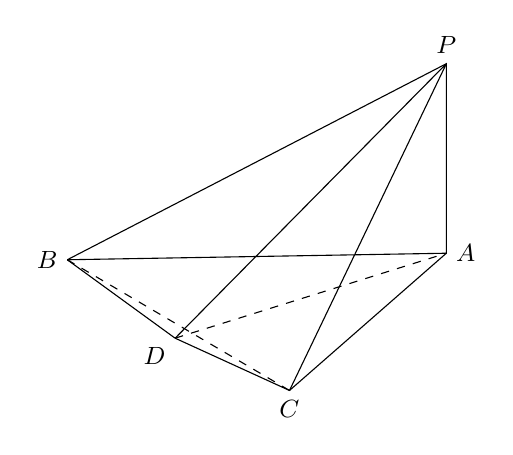
\begin{tikzpicture}[scale=.83, every node/.style={font=\small}]
  \coordinate (B) at (0,2.0);
  \coordinate (D) at (1.65,.8);
  \coordinate (C) at (3.4,0);
  \coordinate (A) at (5.8,2.1);
  \coordinate (P) at (5.8,5.0);
  \draw (B)--(P)--(A)--(C)--(D)--(B);
  \draw (P)--(C) (P)--(D) (B)--(A);
  \draw[dashed] (B)--(C) (D)--(A);
  \node[left] at (B) {$B$};
  \node[below left] at (D) {$D$};
  \node[below] at (C) {$C$};
  \node[right] at (A) {$A$};
  \node[above] at (P) {$P$};
\end{tikzpicture}
